\documentclass[tikz,border=0.1cm]{standalone}
\usepackage{tikz-3dplot}
\usepackage{amsmath,amssymb}
\usepackage{helvet}
\renewcommand{\familydefault}{\sfdefault}

\begin{document}
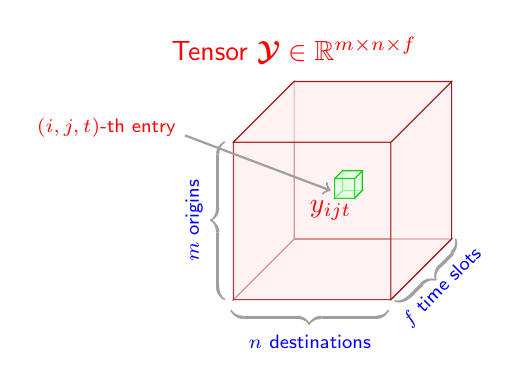
\begin{tikzpicture}[
    cube/.style={draw=#1!60!black, fill=#1!5},
    smallcube/.style={draw=#1!80!black, fill=#1!10},
    label/.style={font=\scriptsize, color=blue},
    brace/.style={color=gray!75},
    tensor/.style={color=red},
    arr/.style={draw=gray!75, thick, ->}
]
% Dimensions
\def\D{2} \def\H{2} \def\W{2} % Main cube
\def\x{1} \def\y{1} \def\z{1}  % Small cube offset
\def\s{0.125}                    % Small cube scale factor

% Main cube
\coordinate (O) at (0,0,0);
\coordinate (A) at (0,\W,0);
\coordinate (B) at (0,\W,\H);
\coordinate (C) at (0,0,\H);
\coordinate (D) at (\D,0,0);
\coordinate (E) at (\D,\W,0);
\coordinate (F) at (\D,\W,\H);
\coordinate (G) at (\D,0,\H);

\draw[cube=red] (O)--(C)--(G)--(D)--cycle; % Bottom
\draw[cube=red] (O)--(A)--(E)--(D)--cycle; % Back
\draw[cube=red] (O)--(A)--(B)--(C)--cycle; % Left
\draw[cube=red,opacity=0.8] (D)--(E)--(F)--(G)--cycle; % Right
\draw[cube=red,opacity=0.6] (C)--(B)--(F)--(G)--cycle; % Front
\draw[cube=red,opacity=0.8] (A)--(B)--(F)--(E)--cycle; % Top

% Small cube
\coordinate (o) at (\x,\y,\z);
\coordinate (a) at (\x,\s*\W+\y,\z);
\coordinate (b) at (\x,\s*\W+\y,\s*\H+\z);
\coordinate (c) at (\x,\y,\s*\H+\z);
\coordinate (d) at (\s*\D+\x,\y,\z);
\coordinate (e) at (\s*\D+\x,\s*\W+\y,\z);
\coordinate (f) at (\s*\D+\x,\s*\W+\y,\s*\H+\z);
\coordinate (g) at (\s*\D+\x,\y,\s*\H+\z);

\draw[smallcube=green] (o)--(c)--(g)--(d)--cycle; % Bottom
\draw[smallcube=green] (o)--(a)--(e)--(d)--cycle; % Back
\draw[smallcube=green] (o)--(a)--(b)--(c)--cycle; % Left
\draw[smallcube=green,opacity=0.8] (d)--(e)--(f)--(g)--cycle; % Right
\draw[smallcube=green,opacity=0.6] (c)--(b)--(f)--(g)--cycle; % Front
\draw[smallcube=green,opacity=0.8] (a)--(b)--(f)--(e)--cycle; % Top

% Labels
\node[label] at (0.2,-1.3,0) {$n$ destinations};
\node[brace] at (0.2,-1,0) {$\underbrace{\hspace{2cm}}$};
\node[label,rotate=90] at (-0.5,1,2) {$m$ origins};
\node[brace,rotate=270] at (-0.2,1,2) {$\underbrace{\hspace{2cm}}$};
\node[label,rotate=45] at (2.5,0,1.6) {$f$ time slots};
\node[brace,rotate=45] at (2.2,0,1.2) {$\underbrace{\hspace{1.1cm}}$};

% Tensor annotation
\draw[arr] (-1,1.7,1) -- (0.85,1,1) node[below,tensor] {$y_{ijt}$};
\node[tensor] at (-2,1.8,1) {\scriptsize $(i,j,t)$-th entry};
\node[tensor] at (0,2.4,0) {Tensor $\boldsymbol{\mathcal{Y}}\in\mathbb{R}^{m\times n\times f}$};

\end{tikzpicture}
\end{document}